\documentclass[a4paper, 14pt]{article}
\usepackage[T2A]{fontenc}
\usepackage[utf8]{inputenc}
\usepackage[russian]{babel}
\usepackage{geometry}
\usepackage{array}
\usepackage{graphicx}
\usepackage{setspace}
\usepackage{siunitx}
\usepackage{caption}
\usepackage{titlesec}
\usepackage{indentfirst}
\usepackage{float}
\usepackage{array}
\usepackage{cellspace}
\usepackage{pgfplots}
\usepackage{pgfplotstable}
\usepackage{tocloft}
\usepackage{amsmath}
\usepackage{multicol}
\usepackage{minted}
\setlength{\cellspacetoplimit}{20pt}
\setlength{\cellspacebottomlimit}{20pt}

\onehalfspacing

\geometry{
  a4paper,
  left=30mm,
  right=20mm,
  top=20mm,
  bottom=20mm
}

\setlength{\parindent}{1.25cm}

\graphicspath{ {images/} }
\captionsetup[figure]{
  labelsep=period,
  justification=centering
}

\renewcommand{\figurename}{Рисунок}
\renewcommand{\contentsname}{Оглавление}

\titleformat{\section}[block]{\normalsize\bfseries}{\thesection}{1em}{}
\titleformat{\subsection}[block]{\normalsize\bfseries}{\thesubsection}{1em}{}
\titlespacing*{\section}{0pt}{\parskip}{-\parskip}
\titlespacing*{\subsection}{0pt}{\parskip}{-\parskip}

\renewcommand{\cftbeforetoctitleskip}{-30pt}
\renewcommand{\cftaftertoctitleskip}{-10pt}

\begin{document}

\begin{titlepage}
  \begin{center}
    \small
    \underline{
      \begin{minipage}{0.2\textwidth}
        \centering
        
\includegraphics[width=3cm]{BMSTU logo}
      \end{minipage}
      \hfill
      \begin{minipage}{0.8\textwidth}
        \begin{center}

          \textbf{Министерство науки и высшего образования Российской Федерации
            Федеральное государственное бюджетное образовательное учреждение высшего образования «Московский государственный технический университет имени Н.Э. Баумана национальный исследовательский университет»
          (МГТУ им. Н.Э. Баумана)}
        \end{center}
      \end{minipage}

    }

    \vspace{7cm}
    \Large
    \textbf{Модульное домашнее задание №1} \\
    \textbf{Вариант 12} \\
    Методы кодирования цифровых данных
    \\
    \vspace{5cm}
    \normalsize
    \begin{tabular}{p{8cm}p{6cm}}
      \textbf{Студент группы ИУ1-31Б} & Соин А. Д. \\
      & «17» апреля 2026 г. \\
      & \\
      \textbf{Преподаватель} & Кузнецов М. А. \\
      & «\underline{\hspace{1.5cm}}»\underline{\hspace{2.5cm}}2025 г. \\
    \end{tabular}
    \vfill{\Large{Москва, 2026}}
  \end{center}
\end{titlepage}

\tableofcontents
\newpage

\section{Методы циклического кодирования}

\subsection{Кодирование исходной последовательности}

Порождающий полином: $g(x) = x^5 + x^2 +1$, в двоичном виде $g(x) = 100101$.

Степень полинома: $r = n - k = 5$.

Сообщение: $46                                                               _{10} = 101110_2$.

Добавляем избыточность: $m(x) = 10111000000_2 $

Деление сообщения на полином: $R = 00010_2$.

Итоговое кодовое слово $c = 10111000010_2$.

\subsection{Построение таблицы синдромов}
\begin{center}
  \begin{table}[H]
    \begin{tabular}{|l|l|l|}
      \hline
      \textbf{i} & $\mathbf{x^i}$ & \textbf{R} \\ \hline
      0 &                              00000000001 &           00001 \\ \hline
      1 &                              00000000010 &           00010 \\ \hline
      2 &                              00000000100 &           00100 \\ \hline
      3 &                              00000001000 &           01000 \\ \hline
      4 &                              00000010000 &           10000 \\ \hline
      5 &                              00000100000 &           00101 \\ \hline
      6 &                              00001000000 &           01010 \\ \hline
      7 &                              00010000000 &           10100 \\ \hline
      8 &                              00100000000 &           01101 \\ \hline
      9 &                              01000000000 &           11010 \\ \hline
      10 &                             10000000000 &           10001 \\ \hline

    \end{tabular}
  \end{table}

\end{center}
\subsection{Моделирование ошибки}

Исходное сообщение: $c = 10111000010_2 $.

Сообщение с ошибкой: $c = 101110\mathbf{1}0010_2 $.

Синдром для данного сообщения: $S(x) = c \bmod g(x) = 10000_2$.

По таблице синдромов ошибка $i = 4$.

Для испраления ошибки произведем операцию $10111010010_2 \oplus 00000010000_2 = 10111000010_2$. Это значение соответствует исходному сообщению, следовательно кодирование проведено верно.

\section{Применение методов физического кодирования}

Для построения временных диаграмм был реализован следующий код matlab.

\begin{minted}{matlab}
  clc; clear; close all;

  %% ---------- Путь сохранения ----------
  scriptPath = fileparts(mfilename('fullpath'));
  if isempty(scriptPath)
      scriptPath = pwd;
  end

  outDir = fullfile(scriptPath, 'results');
  if ~exist(outDir, 'dir')
      mkdir(outDir);
  end

  %% ---------- Исходные данные ----------
  data = [0 0 1 0 1 1 1 0]; % 46 = 00101110 (MSB → LSB)

  Tb = 1;
  samples = 100;

  t = 0:Tb/samples:Tb*length(data)-Tb/samples;

  expand = @(bits) repelem(bits, samples);

  %% ---------- NRZ (однополярный) ----------
  nrz_uni = expand(data);

  figure; stairs(t, nrz_uni, 'LineWidth', 1.5);
  title('NRZ Unipolar'); grid on;
  ylim([-0.5 1.5])
  exportgraphics(gcf, fullfile(outDir,'NRZ_unipolar.png'),'Resolution',300);

  %% ---------- NRZ (биполярный) ----------
  nrz_bi = expand(2*data - 1);

  figure; stairs(t, nrz_bi, 'LineWidth', 1.5);
  title('NRZ Bipolar'); grid on;
  ylim([-1.5 1.5])
  exportgraphics(gcf, fullfile(outDir,'NRZ_bipolar.png'),'Resolution',300);

  %% ---------- NRZ-I (инверсия при 1) ----------
  level = -1;
  nrz_i1 = zeros(1, length(data));
  for i = 1:length(data)
      if data(i) == 1
          level = -level;
      end
      nrz_i1(i) = level;
  end
  nrz_i1 = expand(nrz_i1);

  figure; stairs(t, nrz_i1, 'LineWidth', 1.5);
  title('NRZ-I (инверсия при 1)'); grid on;
  ylim([-1.5 1.5])
  exportgraphics(gcf, fullfile(outDir,'NRZ_I_1.png'),'Resolution',300);

  %% ---------- NRZ-I (инверсия при 0) ----------
  level = -1;
  nrz_i0 = zeros(1, length(data));
  for i = 1:length(data)
      if data(i) == 0
          level = -level;
      end
      nrz_i0(i) = level;
  end
  nrz_i0 = expand(nrz_i0);

  figure; stairs(t, nrz_i0, 'LineWidth', 1.5);
  title('NRZ-I (инверсия при 0)'); grid on;
  ylim([-1.5 1.5])
  exportgraphics(gcf, fullfile(outDir,'NRZ_I_0.png'),'Resolution',300);

  %% ---------- AMI ----------
  ami = zeros(1, length(data));
  level = 1;
  for i = 1:length(data)
      if data(i) == 1
          ami(i) = level;
          level = -level;
      else
          ami(i) = 0;
      end
  end
  ami = expand(ami);

  figure; stairs(t, ami, 'LineWidth', 1.5);
  title('AMI'); grid on;
  ylim([-1.5 1.5])
  exportgraphics(gcf, fullfile(outDir,'AMI.png'),'Resolution',300);

  %% ---------- RZ ----------
  rz = [];
  for i = 1:length(data)
      if data(i) == 1
          rz = [rz ones(1, samples/2), zeros(1, samples/2)];
      else
          rz = [rz -ones(1, samples/2), zeros(1, samples/2)];
      end
  end

  figure; stairs(t, rz, 'LineWidth', 1.5);
  title('RZ'); grid on;
  ylim([-1.5 1.5])
  exportgraphics(gcf, fullfile(outDir,'RZ.png'),'Resolution',300);

  %% ---------- Manchester ----------
  man = [];
  for i = 1:length(data)
      if data(i) == 0
          man = [man ones(1, samples/2), -ones(1, samples/2)];
      else
          man = [man -ones(1, samples/2), ones(1, samples/2)];
      end
  end

  figure; stairs(t, man, 'LineWidth', 1.5);
  title('Manchester (IEEE 802.3)'); grid on;
  ylim([-1.5 1.5])
  exportgraphics(gcf, fullfile(outDir,'Manchester.png'),'Resolution',300);

  %% ---------- Differential Manchester ----------
  diff_man = [];
  level = -1;
  for i = 1:length(data)
      if data(i) == 0
          level = -level;
      end
      first = level;
      second = -level;
      diff_man = [diff_man ...
          first*ones(1, samples/2), ...
          second*ones(1, samples/2)];
      level = second;
  end

  figure; stairs(t, diff_man, 'LineWidth', 1.5);
  title('Differential Manchester'); grid on;
  ylim([-1.5 1.5])
  exportgraphics(gcf, fullfile(outDir,'Diff_Manchester.png'),'Resolution',300);

  %% ---------- 2B1Q ----------
  pairs = reshape(data, 2, [])';
  map = containers.Map({'00','01','10','11'}, [-2.5 -0.833 0.833 2.5]);

  levels = zeros(1, size(pairs,1));
  for i = 1:size(pairs,1)
      key = num2str(pairs(i,:),'%d%d');
      levels(i) = map(key);
  end

  b2q = repelem(levels, samples);
  t2 = 0:Tb/samples:Tb*length(levels)-Tb/samples;

  figure;
  stairs(t2, b2q, 'LineWidth', 1.5);
  title('2B1Q'); grid on;
  ylim([-3.5 3.5])
  exportgraphics(gcf, fullfile(outDir,'2B1Q.png'),'Resolution',300);
\end{minted}

В результате были получены следующие графики

\begin{figure}[H]
  \centering
  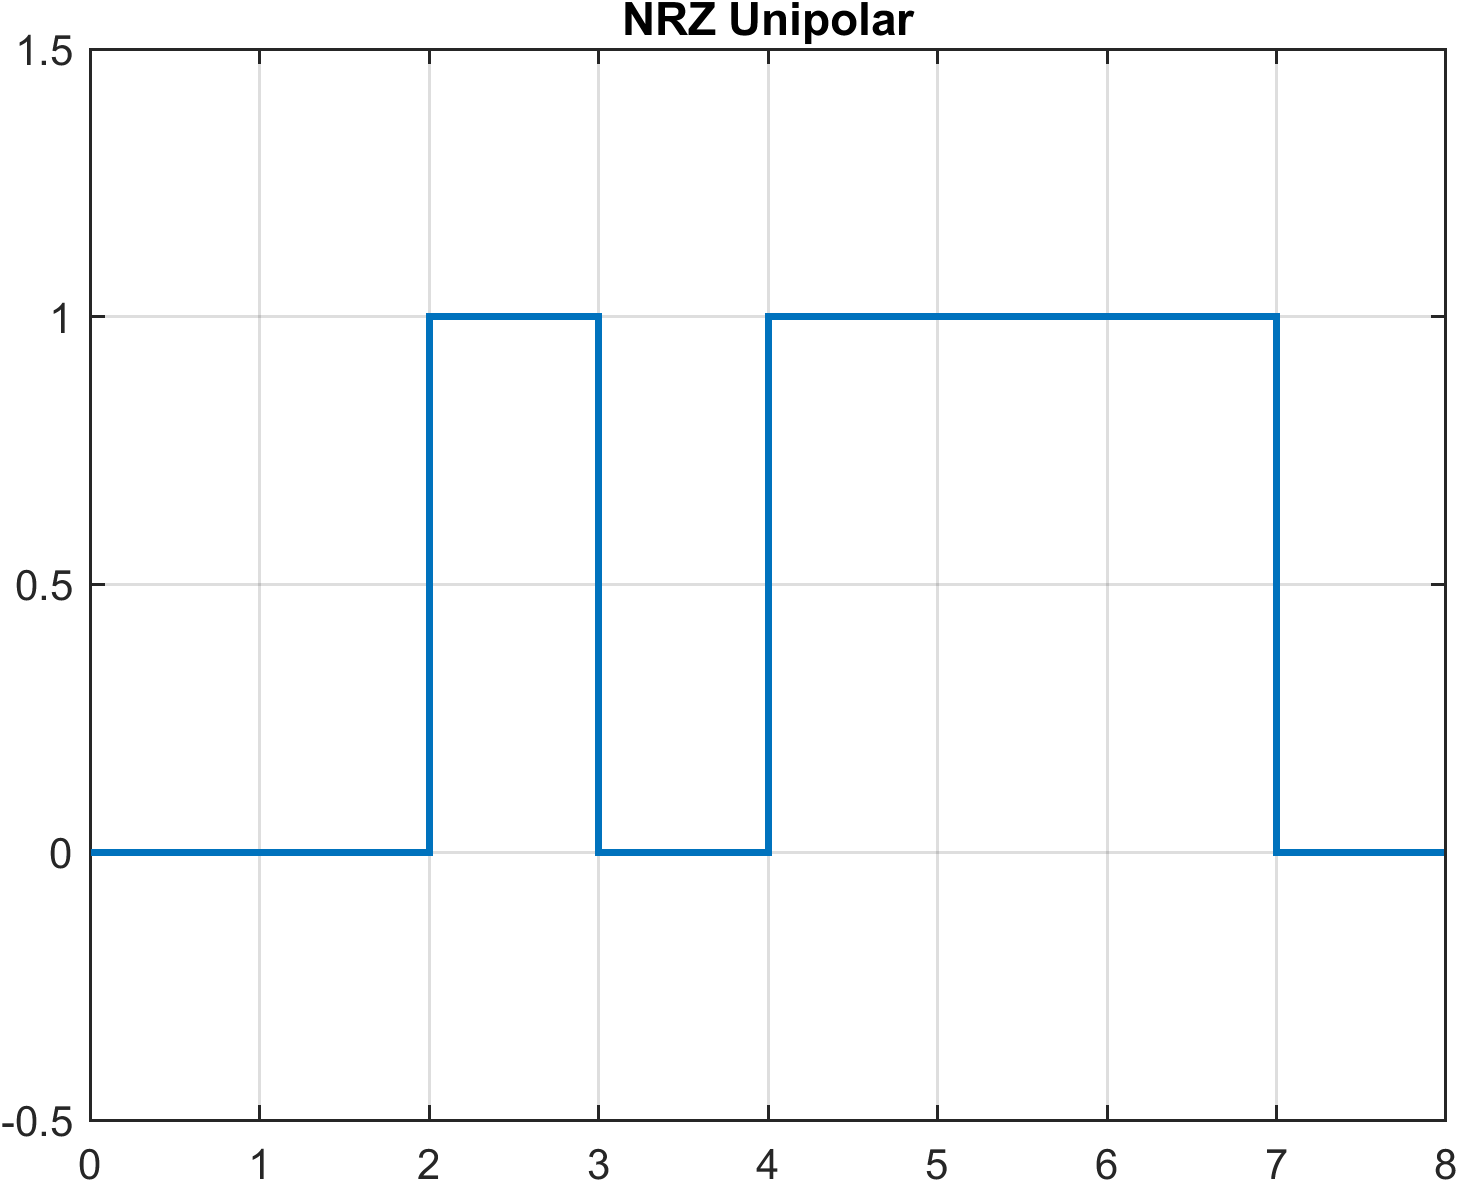
\includegraphics[width=0.8\textwidth]{NRZ_unipolar.png}
  \caption{Код без возвращения к нулю (однополярный)}
\end{figure}

\begin{figure}[H]
  \centering
  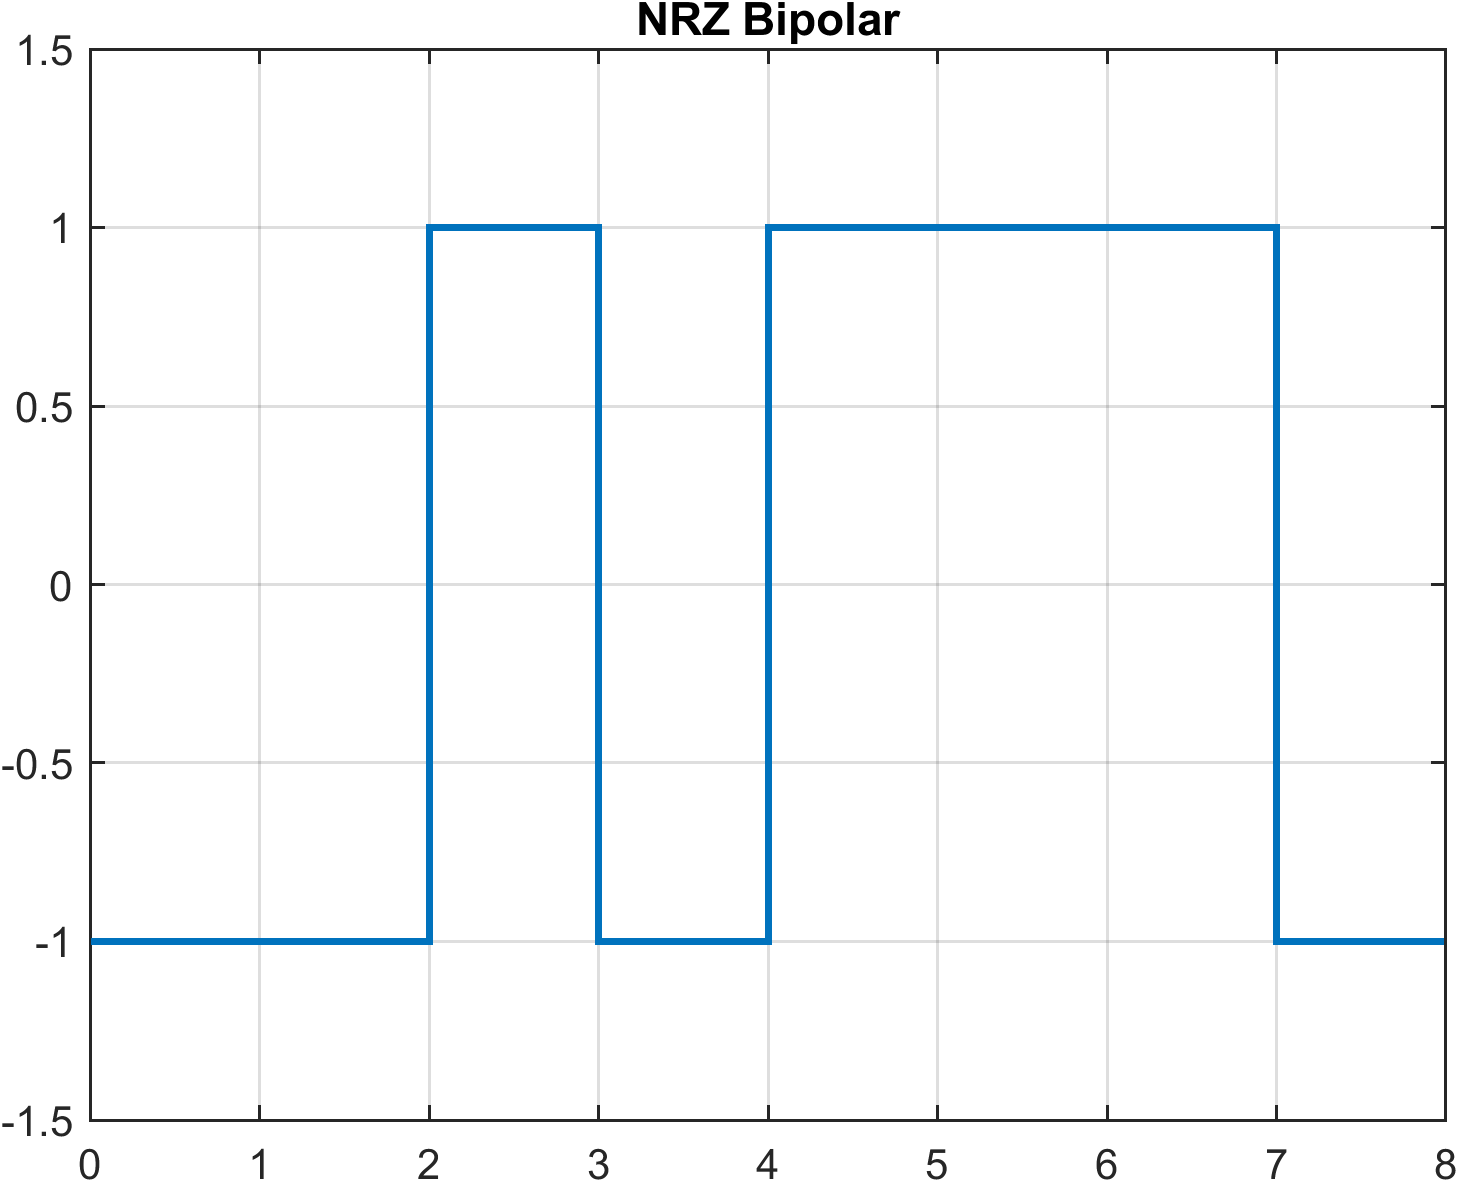
\includegraphics[width=0.8\textwidth]{NRZ_bipolar.png}
  \caption{Код без возвращения к нулю (биполярный)}
\end{figure}

\begin{figure}[H]
  \centering
  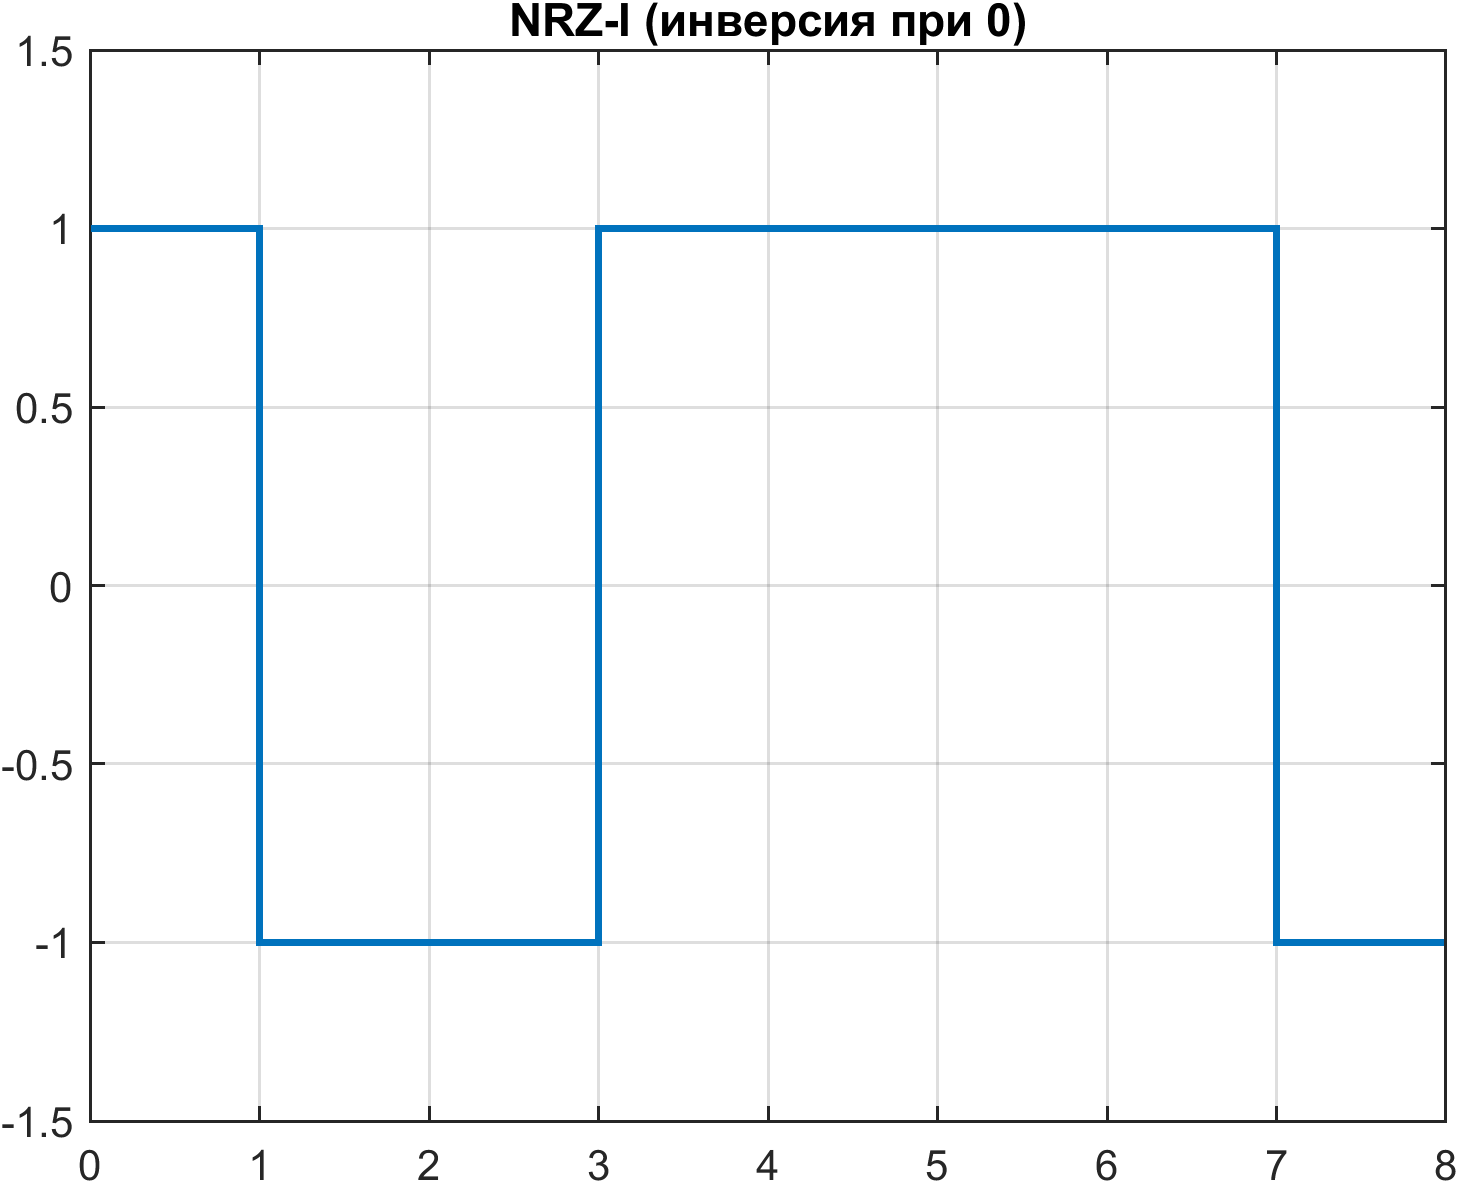
\includegraphics[width=0.8\textwidth]{NRZ_I_0.png}
  \caption{Код без возвращения к нулю с инверсией при нуле}
\end{figure}

\begin{figure}[H]
  \centering
  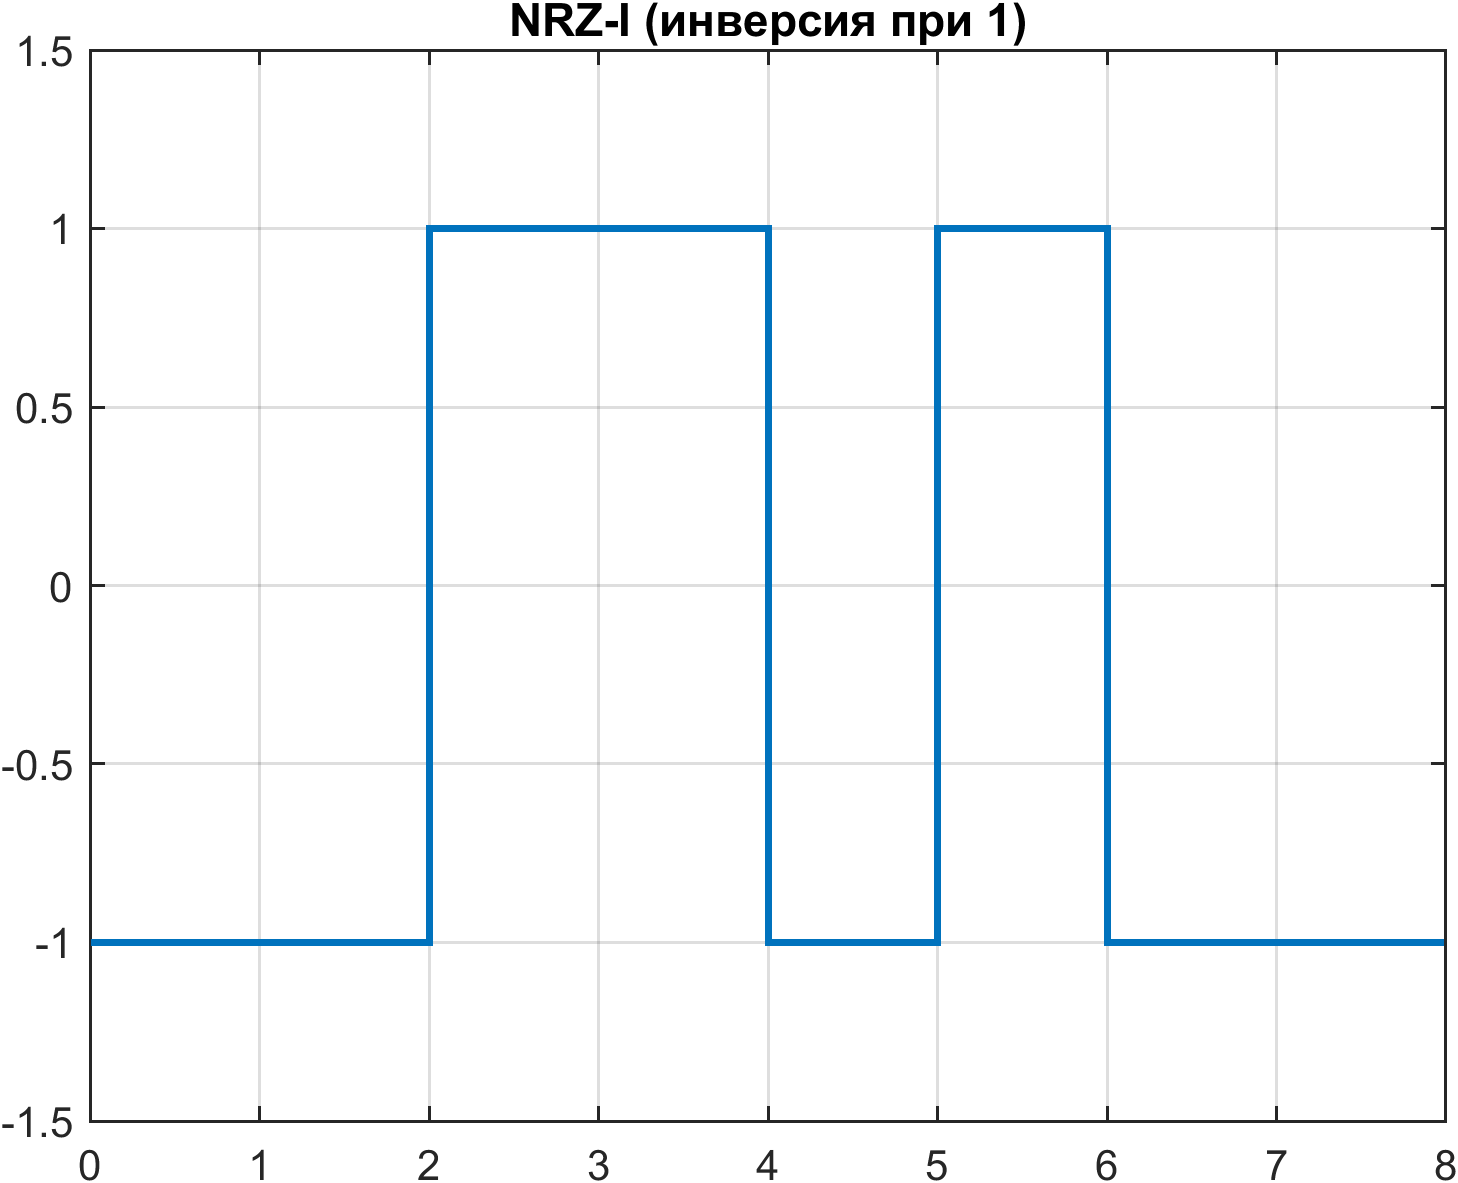
\includegraphics[width=0.8\textwidth]{NRZ_I_1.png}
  \caption{Код без возвращения к нулю с инверсией при единицк}
\end{figure}

\begin{figure}[H]
  \centering
  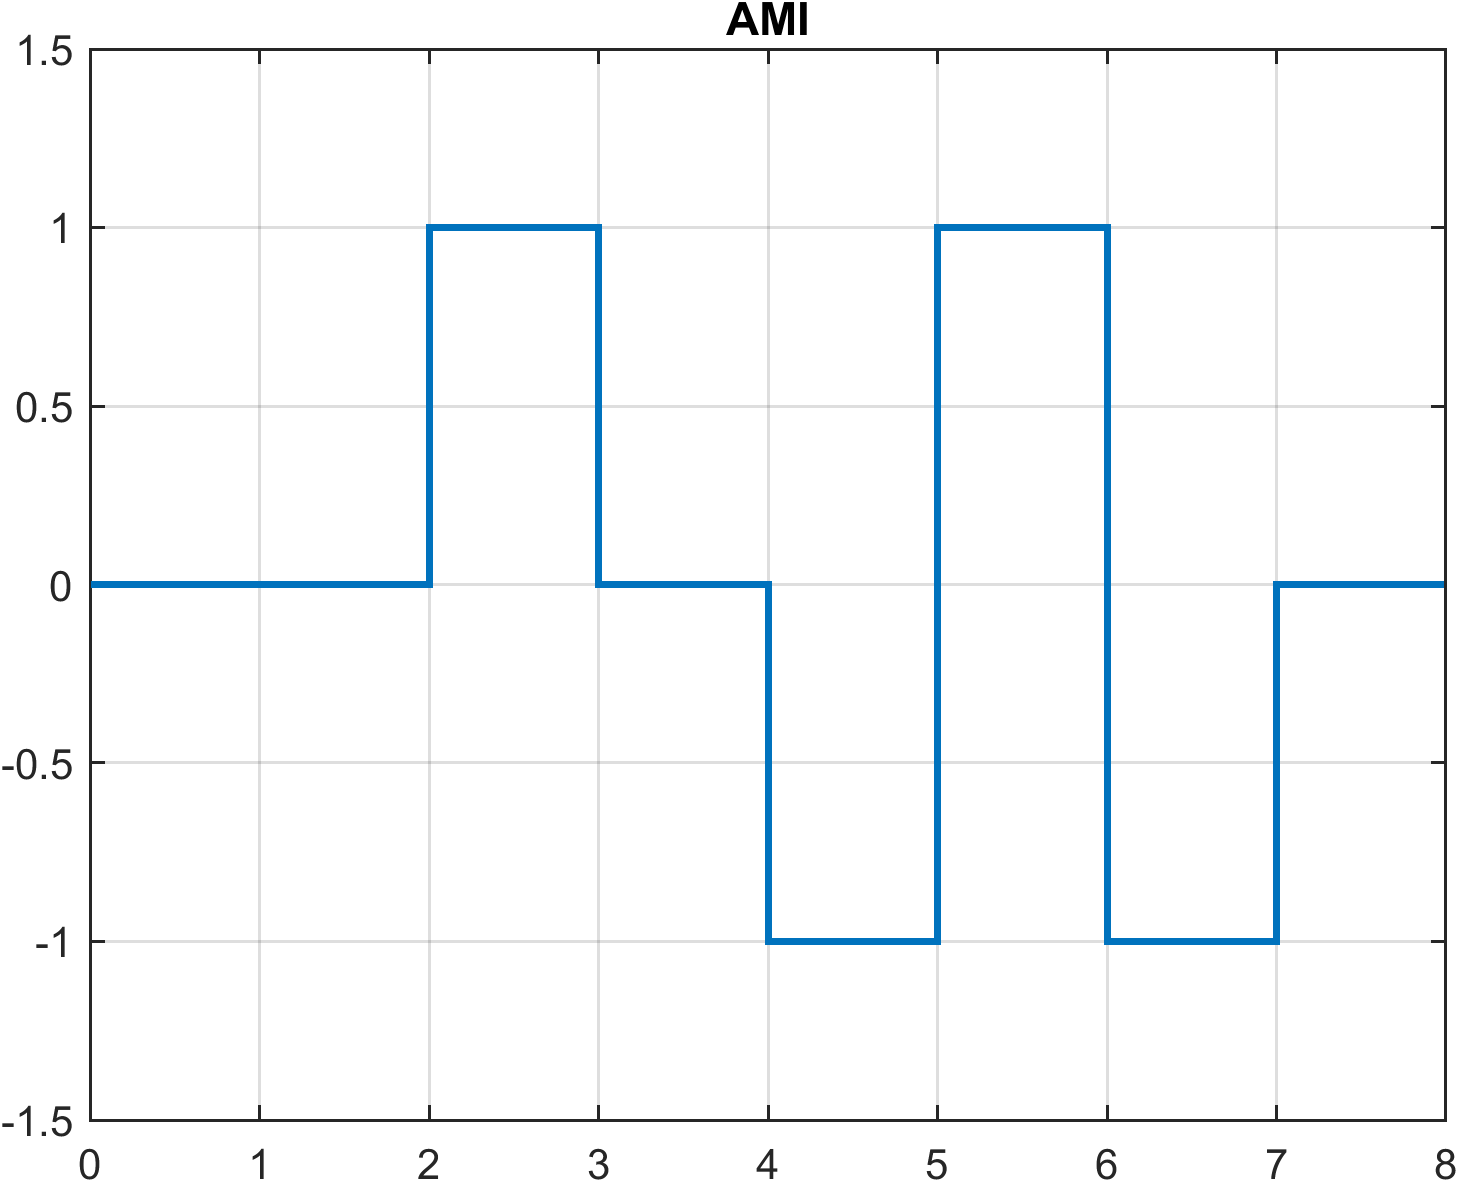
\includegraphics[width=0.8\textwidth]{AMI.png}
  \caption{Код с альтернативной инверсией}
\end{figure}

\begin{figure}[H]
  \centering
  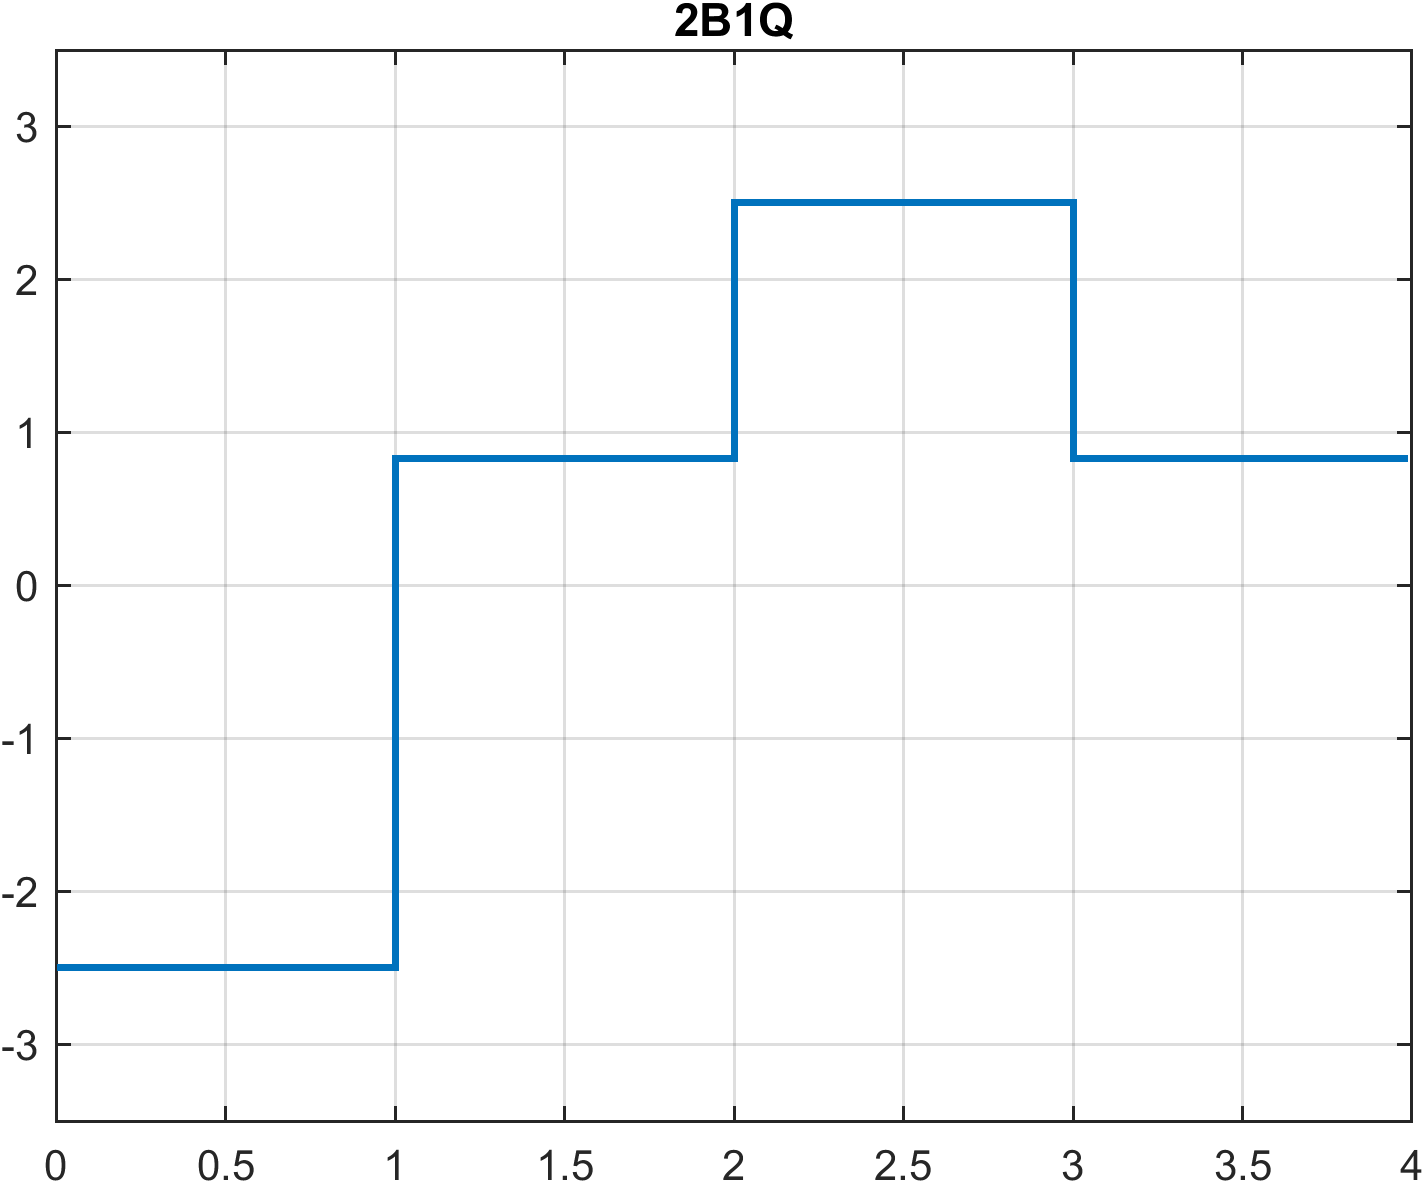
\includegraphics[width=0.8\textwidth]{2B1Q.png}
  \caption{Код 2B1Q}
\end{figure}

\begin{figure}[H]
  \centering
  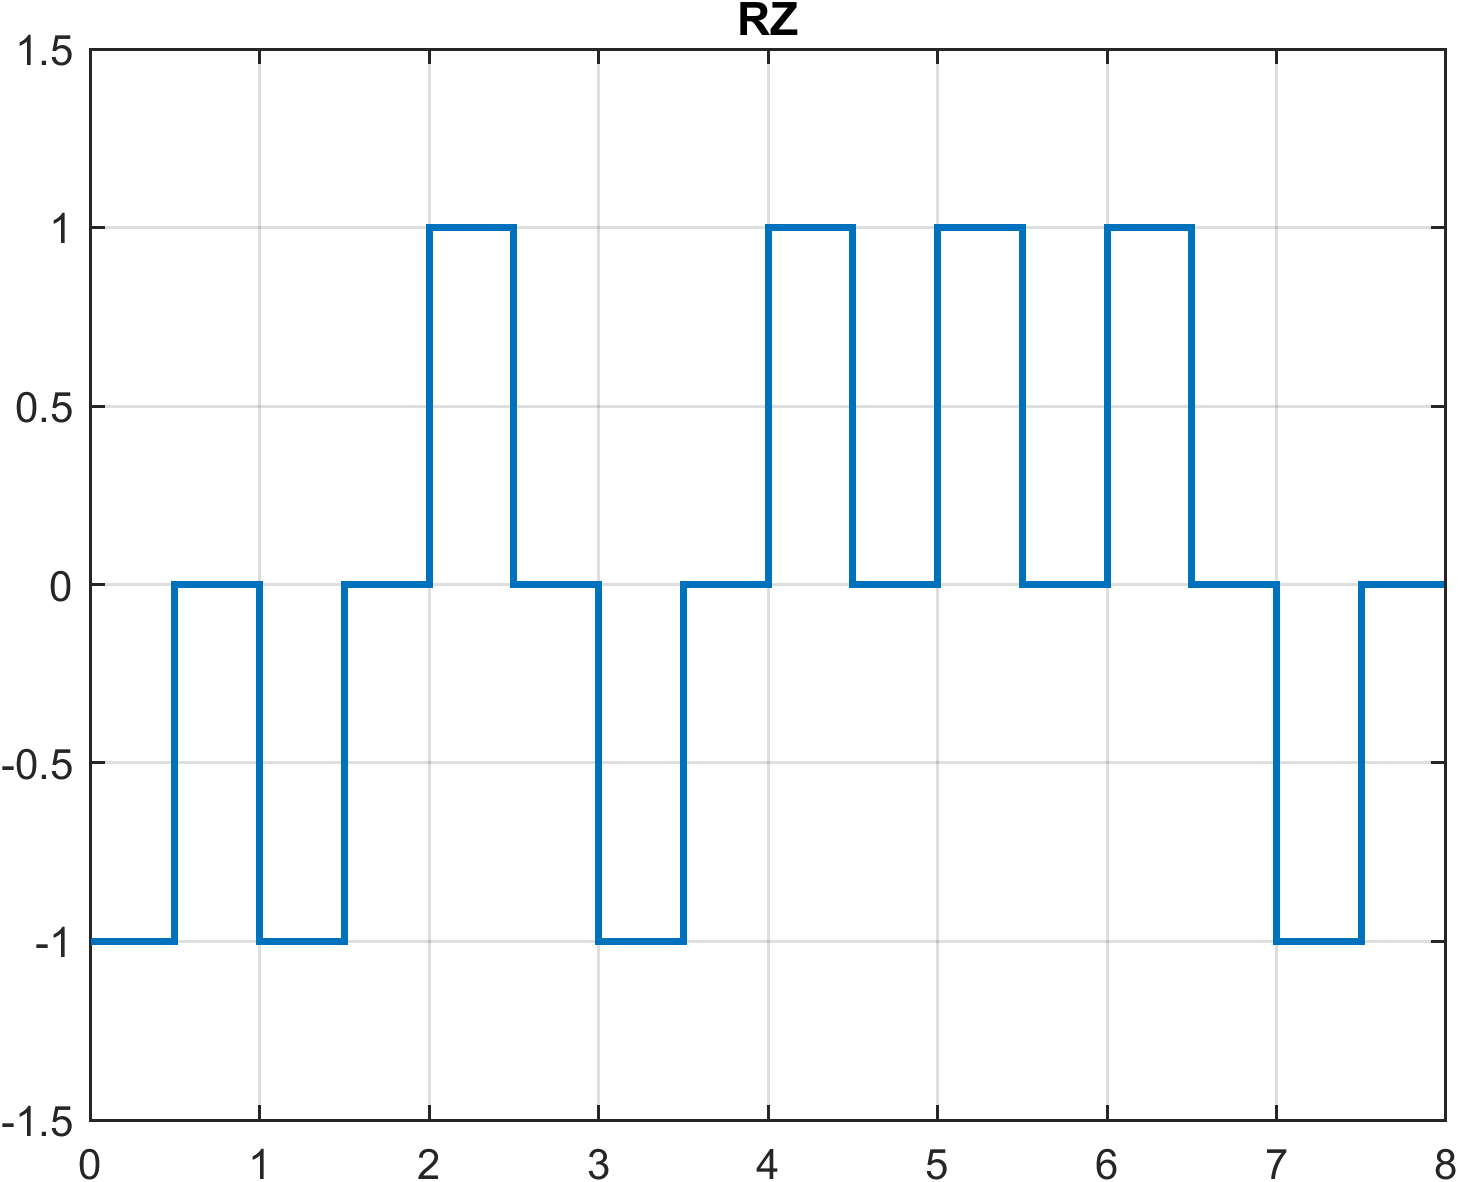
\includegraphics[width=0.8\textwidth]{RZ.png}
  \caption{Код с возвращениемс к нулю}
\end{figure}

\begin{figure}[H]
  \centering
  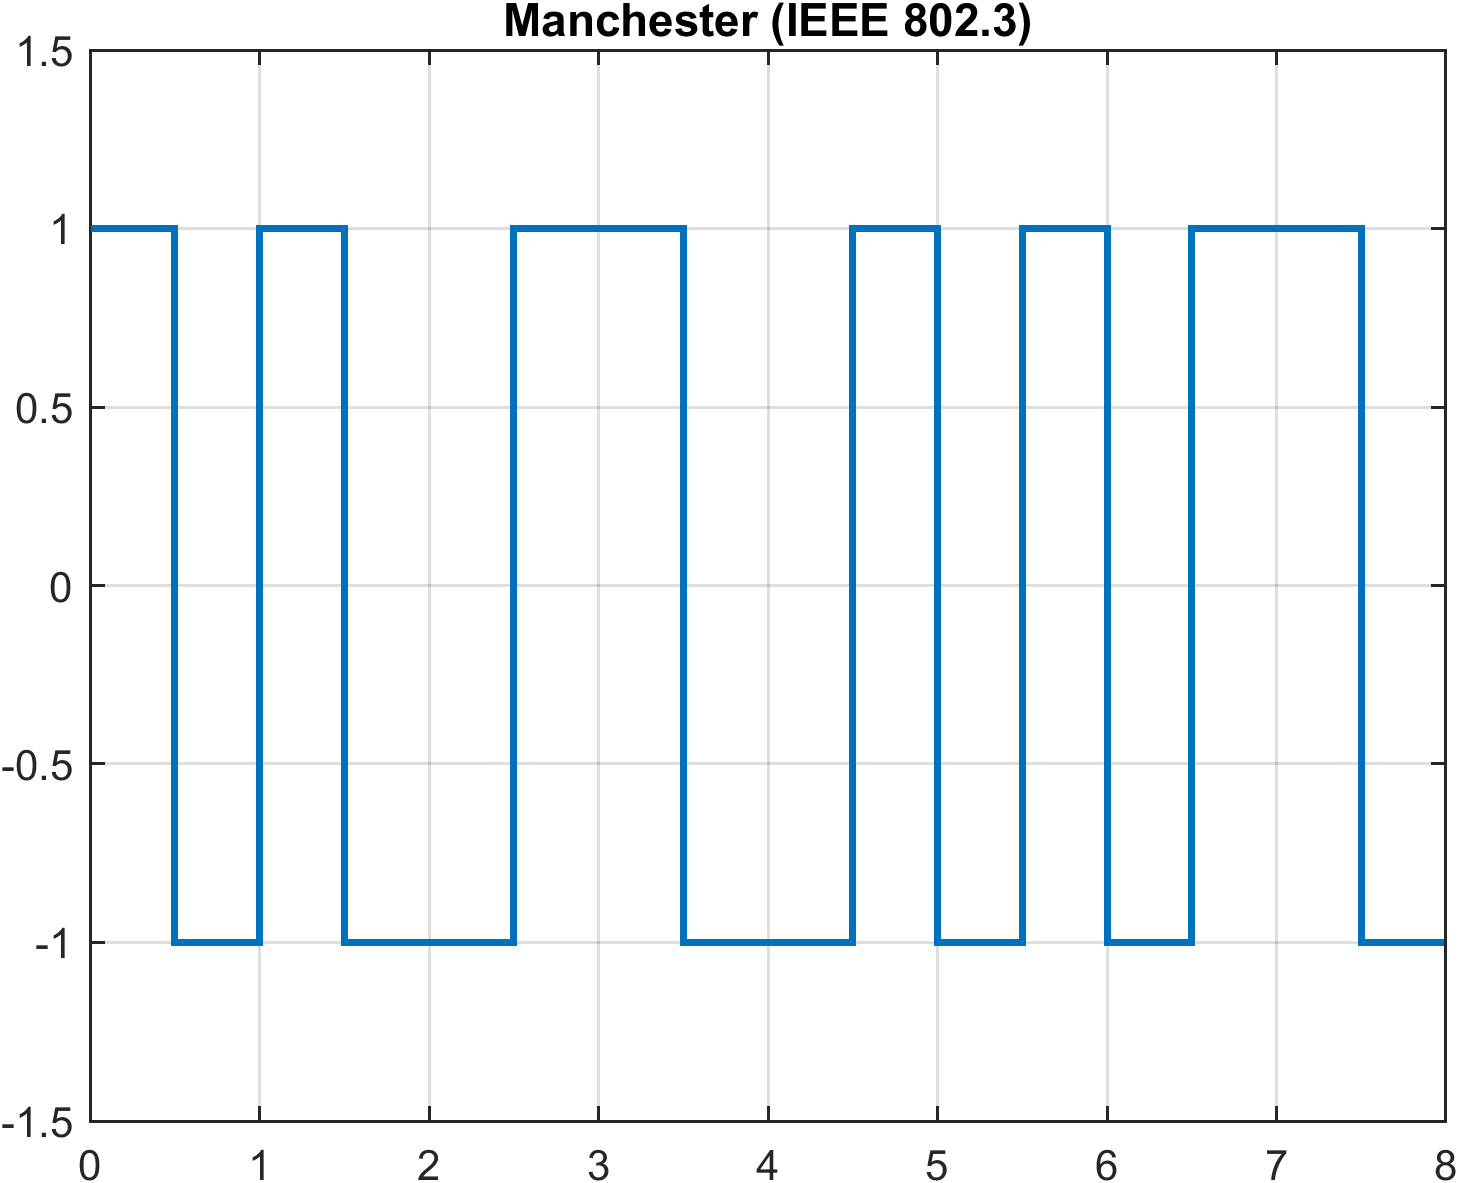
\includegraphics[width=0.8\textwidth]{Manchester.png}
  \caption{Манчестерский код (по стандарту IEEE 802.3)}
\end{figure}

\begin{figure}[H]
  \centering
  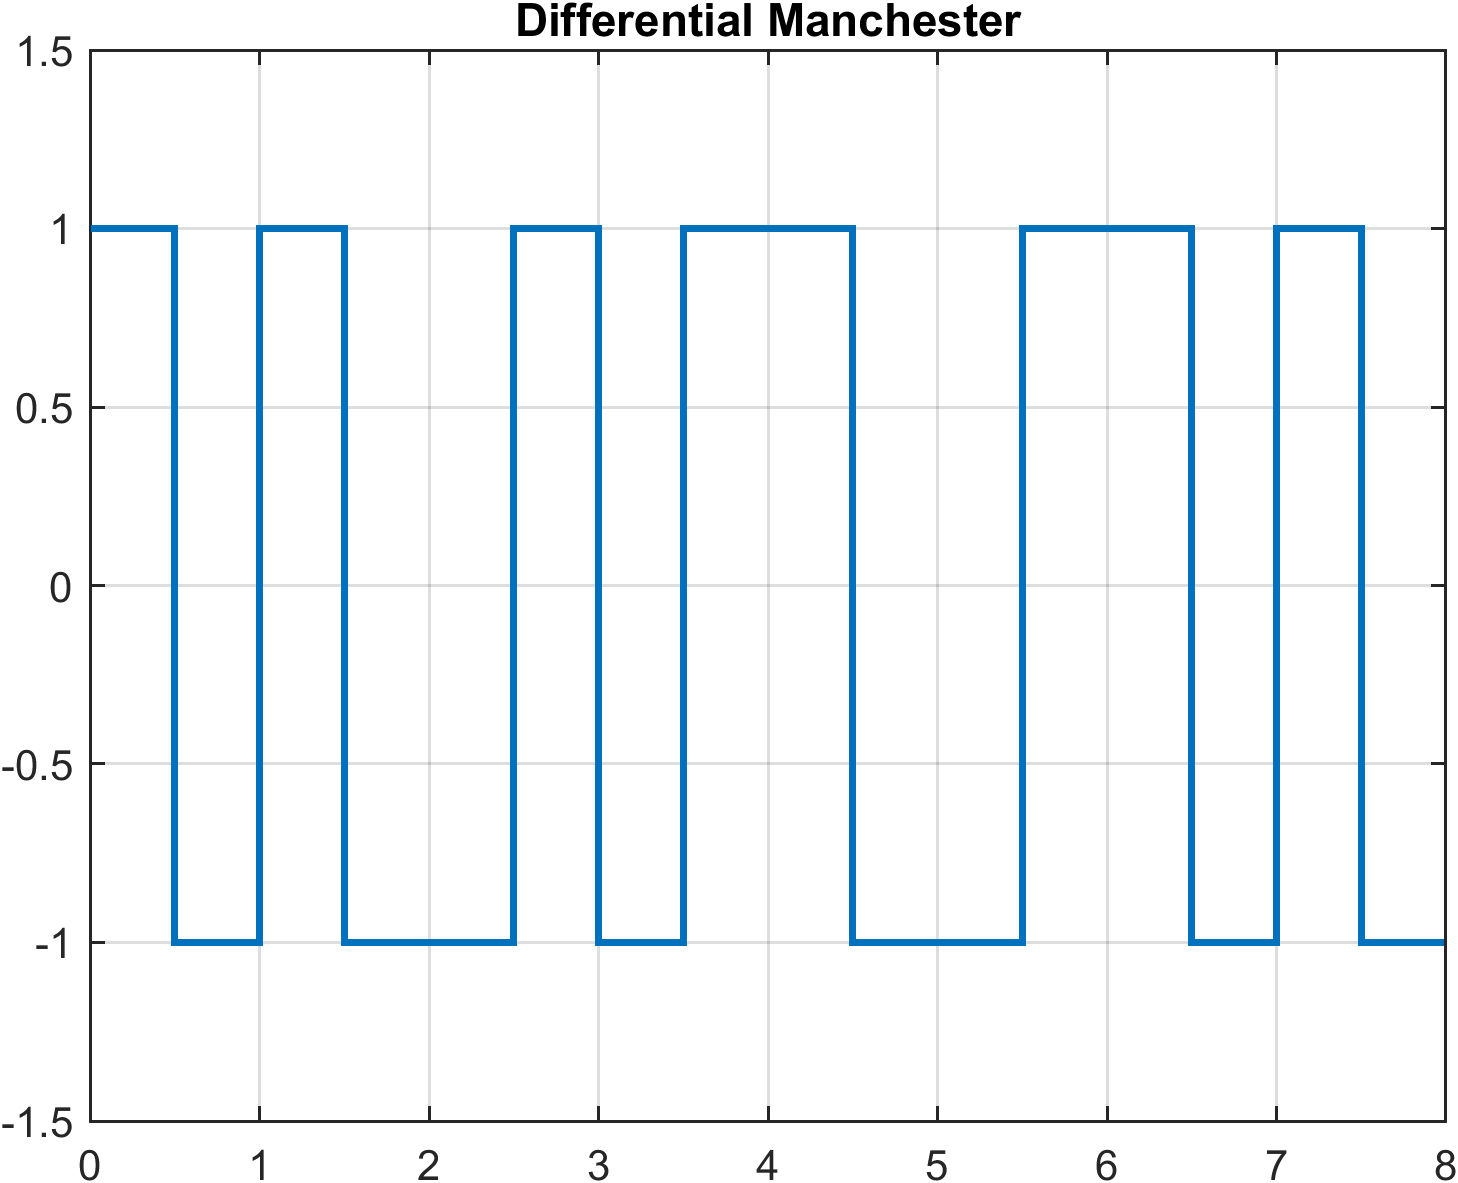
\includegraphics[width=0.8\textwidth]{Diff_Manchester.png}
  \caption{Манчестерский дифференциальный код}
\end{figure}

\end{document}